\documentclass[a4paper,11pt]{article}
% Use ctrl + alt + V to view live pdf

% Packages
\usepackage[utf8]{inputenc} % For encoding
\usepackage[T1]{fontenc} % Better handling of accented characters and hyphenation
\usepackage{microtype} % Improves spacing and justification
\usepackage{amsmath, amssymb} % For equations and symbols
\usepackage{graphicx} % For including graphics/images
\usepackage{caption} % For customizing figure and table captions
\usepackage{subcaption} % For subfigures and subcaptions
\usepackage{float} % For fixing figure and table positions
\usepackage{booktabs} % For professional-looking tables
\usepackage{siunitx} % For consistent typesetting of units and numbers
\usepackage[top=1in, bottom=1in, left=1in, right=1in]{geometry} % Adjusts page margins
\usepackage{fancyhdr} % For custom headers and footers
\usepackage{lmodern} % For a professional-looking font (main body font)
\usepackage{titlesec} % For title customization
\usepackage{array} % For custom table formatting
\usepackage[colorlinks=true, linkcolor=black, urlcolor=black]{hyperref} % Colored links without boxes
\usepackage{cleveref} % For improved cross-referencing    
\usepackage{multirow}
\usepackage{enumitem}
\usepackage{listings}
\usepackage{xcolor}
\usepackage{textcomp}
\usepackage{tabularx}
\usepackage{changepage}
\usepackage{tikz}
\usetikzlibrary{shapes.geometric, arrows}

\lstdefinestyle{python-style}{
    language=Python,
    basicstyle=\ttfamily\footnotesize,
    keywordstyle=\color{blue}\bfseries,
    commentstyle=\color{gray}\itshape,
    stringstyle=\color{green!50!black},
    frame=single,
    breaklines=true,
    showstringspaces=false
}

\lstset{style=python-style}
\lstset{inputpath=Python}
\lstset{captionpos=b}
\lstset{basicstyle=\ttfamily\scriptsize} 
\renewcommand{\lstlistingname}{Program}

% Custom settings
\pagestyle{fancy}
\fancyhf{}
\fancyhead[L]{\textit{SF4 - DataLogger}} % Header left
\fancyhead[R]{\textit{cf573 | wh365}} % Header right 
\fancyfoot[C]{\thepage} % Footer center
\setlength{\headheight}{15pt} % Header height
\setlength{\parindent}{0em} % Indentation for paragraphs
\setlength{\parskip}{0.5em} % Add spacing between paragraphs
\setlength{\abovedisplayskip}{1em}
\setlength{\belowdisplayskip}{1em}
\setlength{\abovedisplayshortskip}{1em}
\setlength{\belowdisplayshortskip}{1em}
% \setlist{topsep=0em, partopsep=0em, itemsep=0em, parsep=0em}

\graphicspath{{Images/}}

\renewcommand{\arraystretch}{1.2}

% Title formatting
\renewcommand{\maketitle}{
    \begin{center}
        \LARGE \textbf{ENGINEERING TRIPOS PART IIA} \\[0.5em]
        \Large \textbf{SF4 – DataLogger} \\[0.5em]
        \textbf{First Interim Report} \\[1.5em]
        \begin{tabularx}{0.7\textwidth}{X X}
            \centering \large Cheng Fang -- cf573 \\ \large Robinson College &
            \centering \large Will Hewes -- wh365 \\ \large Pembroke College
        \end{tabularx}
        \vspace{1em}
    \end{center}
}

\begin{document}
\maketitle
\hrule
\tableofcontents
\newpage

\section{Introduction}
\label{sec:Introduction}

This project aims to develop a microcontroller-based 
automatic plant watering system.
The system will autonomously monitor soil moisture levels, 
plot the data over time, and provide options to water the plant
at scheduled intervals or in response to threshold moisture levels.
This allows for effective monitoring and care with minimal user intervention.

In addition to moisture sensing, the system could be expanded to 
incorporate light and temperature sensors,
enabling further environmental data to be plotted and analysed.
These additional features enhance the system's utility
for controlling the conditions affecting plant health.

\section{Parts List}
\label{sec:Parts_List}

Table \ref{tab:component_order} below displays the components 
ordered to supplement the project so far.
Their usages are discussed further in sections 
\ref{sec:Analogue_Circuit_Design} and \ref{sec:Block_Diagram}.

\begin{table}[H]
    \centering
    \renewcommand{\arraystretch}{1.5}
    \makebox[\linewidth][c]{
    \resizebox{1.1\textwidth}{!}{
    \begin{tabular}{|c|c|c|c|c|}
        \hline
        \textbf{Order Code} & \textbf{Description of Component} & 
        \textbf{Qty} & \textbf{Unit Price (£)} & \textbf{Total Price (£)} \\
        \hline
        2946124 & Capacitive Soil Moisture Sensor Module & 1 & 4.69 & 4.69 \\
        \hline
        SC21096 & Mini servo & 1 & 2.94 & 2.94 \\
        \hline
        4030054 & Temperature sensor & 1 & 1.38 & 1.38 \\
        \hline
    \end{tabular}
    }   
    }
    \caption{Component Order Summary}
    \label{tab:component_order}
\end{table}

\section{Analogue Circuit Design}
\label{sec:Analogue_Circuit_Design}

Figure \ref{fig:Analogue_Circuit_Diagram_for_the_automatic_watering_system}
shows the analogue circuit design for the automatic watering system.

\begin{figure}[H]
    \centering
    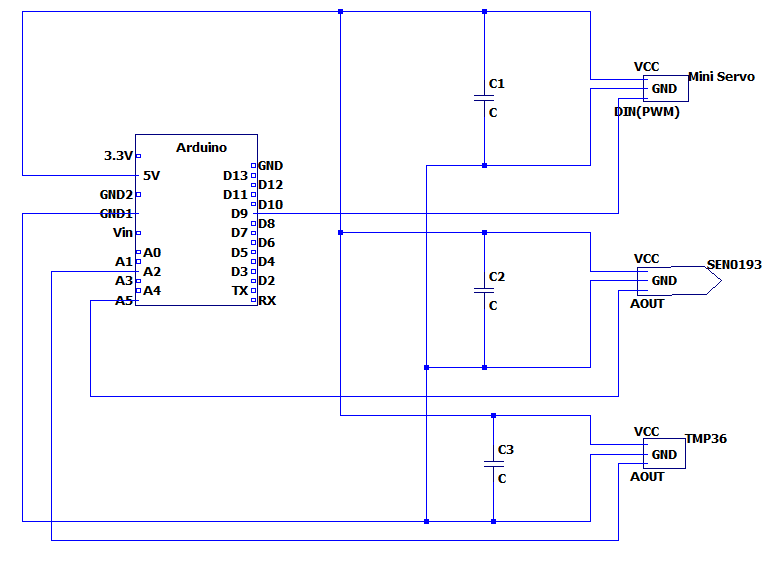
\includegraphics[width=0.6\textwidth]{Analogue Circuit Diagram.png}
    \caption{Analogue Circuit Diagram for the automatic watering system}
    \label{fig:Analogue_Circuit_Diagram_for_the_automatic_watering_system}
\end{figure}

The 5V wire acts as a supply rail, connecting to each of the components,
and routing the ground through where necessary, and 
the I/O pins map to their corresponding components.
Capacitors are added in parallel with each of the sensors
to reduce sensitivity to noise, allowing the data to be tracked
more accurately and eliminating some of the noise.

\section{Block Diagram}
\label{sec:Block_Diagram}

Figure \ref{fig:Block_Diagram_for_the_automatic_watering_system}
shown below displays the general mode of operation for the system.
The sensor modules send real-time information to the Arduino,
which processes and transmits the data to the PC via USB serial communication.

This data is then stored by the PC and displayed graphically in MatLab(?), 
with an interactive GUI through which the 
theshold values, watering timings, or manual watering options
can be controlled by user input.

This is then fed back to the Arduino, 
which will either do nothing if water levels are above the threshold,
or dispense a controlled quantity of water by activating the servo
if moisture levels have fallen below the threshold
(or manual watering is toggled).

\begin{figure}[H]
    \centering
    \includegraphics[width=0.6\textwidth]{DataLogger Block Diagram2.png}
    \caption{Block Diagram for the automatic watering system}
    \label{fig:Block_Diagram_for_the_automatic_watering_system}
\end{figure}

\section{Software Design}
\label{sec:Software_Design}


So far, the software design is in its early stages,
with a mock-up demonstration shown in the Appendix.
The final software implementation will feature 
Arduino communication to the PC via the serial,
plotting capabilities and a GUI,
and an Arduino controlled watering mechanism.

\section{Conclusion}
\label{sec:Conclusion}

The project will work towards building an automated watering system,
capable of logging data with regard to soil moisture levels and temperature.
The key components have been ordered, 
and a preliminary block diagram and circuit design have been constructed - 
though they are subject to change as we test the component properties.

A mock-up software design has been created which allows us to 
simulate an Arduino serial communication and display the current values.
This will be further progressed by implementing 
Arduino communication once the sensors are implemented,
and by enabling plotting, data storage capabilities, and an interactive GUI.

\newpage
\appendix
\section{Software Code}
This software code is just a placeholder to simulate
communication between the Arduino and the PC
before the real system is functional.

\subsection{Sender.py}

\lstinputlisting[
    style=python-style,
    caption={Python script for sending data to the serial port},
    label={Code:sender.py}
]{sender.py}

\subsection{Receiver.py}

\lstinputlisting[
    style=python-style,
    caption={Python script for receiving sending data to the serial port},
    label={Code:receiver.py}
]{receiver.py}

\end{document}